\documentclass[10pt,a4paper]{article}

% ==============================================================================
%  PACKAGE IMPORTS & ENGINE CONFIGURATION
% ==============================================================================
\usepackage[utf8]{inputenc}
\usepackage[T1]{fontenc}
\usepackage{geometry}
\geometry{
  a4paper,
  top=18mm,
  bottom=18mm,
  left=16mm,
  right=16mm,
  headheight=18pt,
  headsep=8pt,
  footskip=12pt
}

% Typography
\usepackage{mathpazo}            % Palatino body font
\usepackage[scaled=0.92]{helvet}  % Clean sans-serif for headers
\usepackage[scaled=0.86]{inconsolata} % Monospace font for code
\usepackage{microtype}
\usepackage{amsmath,amssymb,amsthm}

% Colors & Graphics
\usepackage[table,xcdraw,dvipsnames]{xcolor}
\usepackage{graphicx}
\usepackage{tikz}
\usetikzlibrary{arrows.meta,positioning,shapes.geometric,shadows,calc,fit,backgrounds}
\usepackage{booktabs}
\usepackage{tabularx}
\usepackage{array}
\usepackage{fancyhdr}
\usepackage{lastpage}
\usepackage{float}
\usepackage{caption}

% Code Listings & Callout Boxes
\usepackage{listings}
\usepackage[many]{tcolorbox}
\tcbuselibrary{listings,skins,breakable}

% Hyperref (Loaded late)
\usepackage[
  colorlinks=true,
  linkcolor=brandblue,
  citecolor=brandteal,
  urlcolor=brandblue,
  bookmarksnumbered=true,
  pdfstartview=FitH
]{hyperref}

% ==============================================================================
%  PROFESSIONAL COLOR PALETTE (DEEP NAVY & SLATE ARCHITECTURAL SYSTEM)
% ==============================================================================
\definecolor{brandnavy}{HTML}{0B192C}     % Deep Obsidian Navy
\definecolor{brandblue}{HTML}{1E3E62}     % Slate Steel Blue
\definecolor{brandteal}{HTML}{008080}     % Deep Teal Accent
\definecolor{brandaccent}{HTML}{E57373}   % Coral Alert
\definecolor{brandgreen}{HTML}{2E7D32}    % Validated Emerald
\definecolor{branddark}{HTML}{1A1A24}     % Charcoal Body Text
\definecolor{brandcard}{HTML}{F8FAFC}     % Clean Slate Background
\definecolor{brandsurface}{HTML}{F1F5F9}  % Light Box Surface
\definecolor{brandborder}{HTML}{CBD5E1}   % Border Slate Grey
\definecolor{codebg}{HTML}{F8FAFC}        % Code Editor Background
\definecolor{codekw}{HTML}{0F4C81}        % Code Keyword (Classic Blue)
\definecolor{codestr}{HTML}{1E6B52}       % Code String (Muted Forest)
\definecolor{codecomm}{HTML}{64748B}      % Code Comment (Slate Neutral)
\definecolor{codenum}{HTML}{94A3B8}       % Line Number Gutter

% ==============================================================================
%  LISTINGS & TCOLORBOX STYLING
% ==============================================================================
\lstdefinestyle{AetherPython}{
  language=Python,
  basicstyle=\fontsize{7.4}{9.4}\ttfamily\color{branddark},
  keywordstyle=\bfseries\color{codekw},
  stringstyle=\color{codestr},
  commentstyle=\itshape\color{codecomm},
  numberstyle=\tiny\color{codenum},
  numbers=left,
  numbersep=7pt,
  stepnumber=1,
  breaklines=true,
  breakatwhitespace=false,
  showstringspaces=false,
  tabsize=4,
  columns=fullflexible,
  keepspaces=true,
  upquote=true,
  frame=none
}

\newtcolorbox{codebox}[2][]{
  enhanced,
  colback=codebg,
  colframe=brandborder,
  boxrule=0.7pt,
  arc=3pt,
  top=3pt, bottom=3pt, left=3pt, right=3pt,
  title={\sffamily\scriptsize\bfseries\color{brandnavy}#2},
  coltitle=brandnavy,
  colbacktitle=brandsurface,
  titlerule=0.5pt,
  titlerule style=brandborder,
  #1
}

\newtcolorbox{specbox}[2][]{
  enhanced,
  colback=brandcard,
  colframe=brandblue,
  boxrule=1.0pt,
  arc=3pt,
  fonttitle=\sffamily\bfseries\small,
  title={#2},
  top=5pt, bottom=5pt, left=8pt, right=8pt,
  #1
}

\newtcolorbox{proofbox}[2][]{
  enhanced,
  colback=brandsurface,
  colframe=brandteal,
  boxrule=1.0pt,
  arc=3pt,
  fonttitle=\sffamily\bfseries\small,
  title={#2},
  top=4pt, bottom=4pt, left=8pt, right=8pt,
  #1
}

% ==============================================================================
%  PAGE HEADERS & FOOTERS
% ==============================================================================
\pagestyle{fancy}
\fancyhf{}
\renewcommand{\headrulewidth}{0.5pt}
\renewcommand{\footrulewidth}{0.5pt}
\renewcommand{\headrule}{\hbox to\headwidth{\color{brandborder}\leaders\hrule height \headrulewidth\hfill}}
\renewcommand{\footrule}{\hbox to\headwidth{\color{brandborder}\leaders\hrule height \footrulewidth\hfill}}

\fancyhead[L]{\sffamily\scriptsize\bfseries\color{brandnavy}AETHERGRID-AI \textbar\ CORE ENGINE SPECIFICATION}
\fancyhead[C]{\sffamily\scriptsize\color{codecomm}Dynamic Cost Pricing \& Traversal Engine}
\fancyhead[R]{\sffamily\scriptsize\color{brandnavy}UCS503P Software Engineering}

\fancyfoot[L]{\sffamily\scriptsize\color{codecomm}AetherGrid-AI Core Engine \textbar\ Dynamic Cost Pricing \& Traversal}
\fancyfoot[C]{}
\fancyfoot[R]{\sffamily\scriptsize\bfseries\color{brandnavy}Page \thepage\ of \pageref{LastPage}}

% Section title styling
\usepackage{titlesec}
\titleformat{\section}
  {\sffamily\Large\bfseries\color{brandnavy}}
  {\thesection}{1em}{}
  [\color{brandteal}\rule{0.25\textwidth}{1.2pt}]

\titleformat{\subsection}
  {\sffamily\large\bfseries\color{brandblue}}
  {\thesubsection}{0.8em}{}

\titleformat{\subsubsection}
  {\sffamily\normalsize\bfseries\color{brandnavy}}
  {\thesubsubsection}{0.6em}{}

\titlespacing*{\section}{0pt}{8pt}{4pt}
\titlespacing*{\subsection}{0pt}{6pt}{3pt}
\titlespacing*{\subsubsection}{0pt}{5pt}{2pt}

\setlength{\parskip}{3.5pt}
\setlength{\parindent}{0pt}
\setlength{\abovedisplayskip}{3pt}
\setlength{\belowdisplayskip}{3pt}

\begin{document}

% ==============================================================================
%  PAGE 1: BANNER, ABSTRACT, SYSTEM ARCHITECTURE & COMPONENT DIAGRAM
% ==============================================================================
\begin{tcolorbox}[
  enhanced,
  colback=brandnavy,
  colframe=brandnavy,
  arc=4pt,
  boxrule=0pt,
  top=10pt, bottom=10pt, left=14pt, right=14pt,
  drop shadow={opacity=0.15}
]
  \begin{minipage}{0.73\textwidth}
    {\fontsize{19}{23}\sffamily\bfseries\color{white}AetherGrid-AI Core Engine}\\[3pt]
    {\large\sffamily\color{brandsurface}Dynamic Cost Pricing \& Traversal Engine --- Code Documentation}\\[4pt]
    {\footnotesize\sffamily\color{brandborder}Production Architecture: Time-Dependent Edge Pricing, Heuristic Admissibility, Anti-Flapping Filters, and Invariant Verification}
  \end{minipage}
  \hfill
  \begin{minipage}{0.25\textwidth}
    \raggedleft
    {\sffamily\scriptsize\color{brandaccent}\textbf{Course}: UCS503P (SE)}\\[1.5pt]
    {\sffamily\scriptsize\color{brandborder}\textbf{Date}: September 2026}\\[1.5pt]
    {\sffamily\scriptsize\color{brandborder}\textbf{Status}: Phase 01 Validated}\\[1.5pt]
    {\sffamily\scriptsize\color{brandborder}\textbf{Package}: \texttt{Aether/core/}}
  \end{minipage}
\end{tcolorbox}

\vspace{1pt}

\begin{tcolorbox}[
  enhanced,
  colback=brandsurface,
  colframe=brandborder,
  boxrule=0.6pt,
  arc=3pt,
  top=5pt, bottom=5pt, left=10pt, right=10pt
]
  \sffamily\small
  \textbf{Authors}: Vishal Singla (1024240009) \& Sparsh Verma (1024240011) \hfill \textbf{Affiliation}: Thapar Institute of Engineering \& Technology \\[2pt]
  \textbf{Abstract \& Purpose}: In emergency autonomous dispatch, the routing engine's path quality and convergence rate depend entirely on the dynamic edge pricing function $c(e, t)$. If costs fail to capture real-time bottlenecks, fleet vehicles enter gridlock; if costs fluctuate with high-frequency sensor updates, routing decisions suffer from catastrophic \textit{route flapping}; if heuristic lower bounds overestimate travel times, $A^*$ search forfeits mathematical optimality. This specification documents the implementation of \texttt{Aether.core.pricing} and its dependencies, providing the mathematical derivations, production code snippets, architectural dataflow schematics, formal admissibility proofs, and unit test verification.
\end{tcolorbox}

\section{System Architecture \& Module Decomposition}

The Aether dispatch backend is structured as a modular, time-varying directed graph system located in \texttt{Aether/core/}. The cost pricing engine (\texttt{pricing.py}) acts as the centralized evaluator connecting environmental state, vehicular density, and road topography.

\subsection{Component Dependency Architecture}
Figure~\ref{fig:architecture} illustrates the architectural dependency hierarchy and data contracts between modules. During graph search, the traversal engine queries \texttt{calculate\_edge\_cost()} across open frontiers while using \texttt{compute\_admissible\_heuristic()} for priority queue ordering.

\begin{figure}[H]
\centering
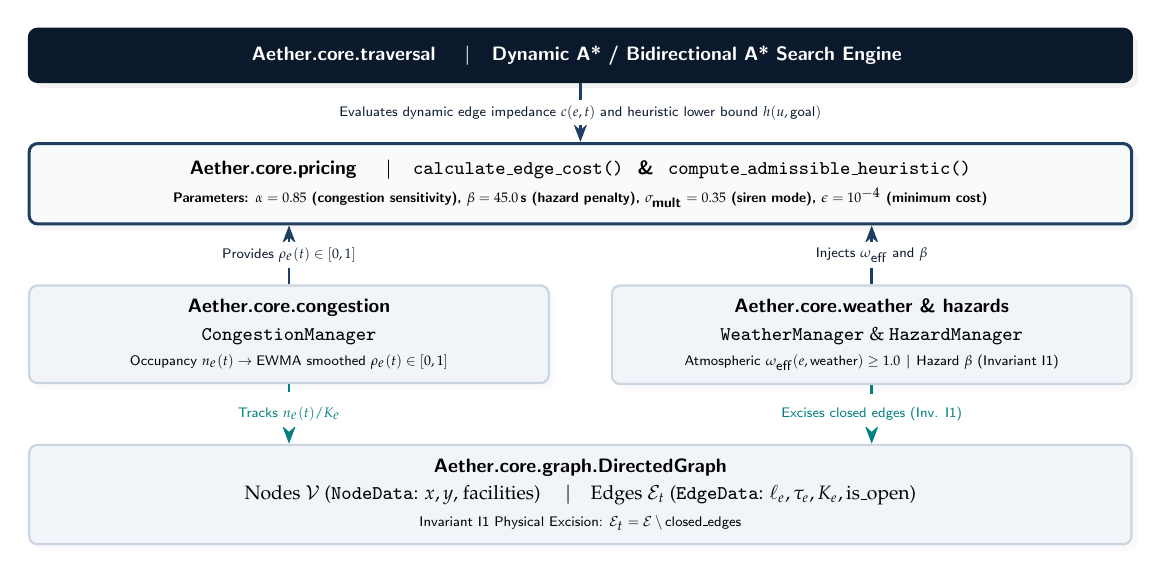
\begin{tikzpicture}[
  node distance=0.65cm and 0.8cm,
  box/.style={
    draw=brandborder, fill=brandsurface, rounded corners=3pt, line width=0.8pt,
    font=\sffamily\scriptsize, align=center, inner sep=5pt, drop shadow={opacity=0.04}
  },
  corebox/.style={
    draw=brandblue, fill=brandcard, rounded corners=3pt, line width=1.1pt,
    font=\sffamily\scriptsize\bfseries, align=center, inner sep=6pt, drop shadow={opacity=0.08}
  },
  enginebox/.style={
    draw=brandnavy, fill=brandnavy, rounded corners=3pt, line width=1.0pt,
    font=\sffamily\scriptsize\bfseries\color{white}, align=center, inner sep=6pt, drop shadow={opacity=0.10}
  },
  arrow/.style={-{Stealth[scale=0.85]}, line width=1.0pt, draw=brandblue}
]
  % Layer 1: Traversal Engine (Top)
  \node[enginebox, minimum width=14.0cm] (traversal) {
    \textbf{Aether.core.traversal} \quad\textbar\quad Dynamic A* / Bidirectional A* Search Engine
  };

  % Layer 2: Pricing Engine (Central Evaluator)
  \node[corebox, below=0.75cm of traversal, minimum width=14.0cm] (pricing) {
    \textbf{Aether.core.pricing} \quad\textbar\quad \texttt{calculate\_edge\_cost()} \ \& \ \texttt{compute\_admissible\_heuristic()}\\[2pt]
    \tiny Parameters: $\alpha = 0.85$ (congestion sensitivity), $\beta = 45.0\,\text{s}$ (hazard penalty), $\sigma_{\text{mult}} = 0.35$ (siren mode), $\epsilon = 10^{-4}$ (minimum cost)
  };

  % Layer 3: Two State Managers (Left and Right)
  \node[box, below=0.75cm of pricing, xshift=-3.7cm, minimum width=6.6cm] (congestion) {
    \textbf{Aether.core.congestion}\\[2pt]
    \normalfont\scriptsize \texttt{CongestionManager}\\[1pt]
    \tiny Occupancy $n_e(t) \to \text{EWMA smoothed } \rho_e(t) \in [0, 1]$
  };

  \node[box, below=0.75cm of pricing, xshift=3.7cm, minimum width=6.6cm] (environment) {
    \textbf{Aether.core.weather \& hazards}\\[2pt]
    \normalfont\scriptsize \texttt{WeatherManager} \& \texttt{HazardManager}\\[1pt]
    \tiny Atmospheric $\omega_{\text{eff}}(e, \text{weather}) \ge 1.0$ \textbar\ Hazard $\beta$ (Invariant I1)
  };

  % Layer 4: Foundation Graph
  \node[box, below=0.75cm of $(congestion.south)!0.5!(environment.south)$, minimum width=14.0cm] (graph) {
    \textbf{Aether.core.graph.DirectedGraph}\\[2pt]
    \normalfont\scriptsize Nodes $\mathcal{V}$ (\texttt{NodeData}: $x, y$, facilities) \quad\textbar\quad Edges $\mathcal{E}_t$ (\texttt{EdgeData}: $\ell_e, \tau_e, K_e, \text{is\_open}$)\\[1.5pt]
    \tiny Invariant I1 Physical Excision: $\mathcal{E}_t = \mathcal{E} \setminus \text{closed\_edges}$
  };

  % Clean vertical dataflow arrows
  \draw[arrow] (traversal.south) -- node[fill=white, inner sep=2pt, font=\sffamily\tiny\color{brandnavy}] {Evaluates dynamic edge impedance $c(e, t)$ and heuristic lower bound $h(u, \text{goal})$} (pricing.north);

  \draw[arrow] (congestion.north) -- node[fill=white, inner sep=2pt, font=\sffamily\tiny\color{brandnavy}] {Provides $\rho_e(t) \in [0, 1]$} (congestion.north |- pricing.south);
  \draw[arrow] (environment.north) -- node[fill=white, inner sep=2pt, font=\sffamily\tiny\color{brandnavy}] {Injects $\omega_{\text{eff}}$ and $\beta$} (environment.north |- pricing.south);

  \draw[arrow, dashed, draw=brandteal] (congestion.south) -- node[fill=white, inner sep=2pt, font=\sffamily\tiny\color{brandteal}] {Tracks $n_e(t) / K_e$} (congestion.south |- graph.north);
  \draw[arrow, dashed, draw=brandteal] (environment.south) -- node[fill=white, inner sep=2pt, font=\sffamily\tiny\color{brandteal}] {Excises closed edges (Inv. I1)} (environment.south |- graph.north);
\end{tikzpicture}
\caption{System Component Architecture: Layered dataflow hierarchy from traversal engine to physical graph.}
\label{fig:architecture}
\end{figure}

\newpage
% ==============================================================================
%  PAGE 2: DATA MODELS, TABLE 1, MATHEMATICAL PRICING & API SPECIFICATION
% ==============================================================================
\subsection{Core Data Models \& Graph Contracts (\texttt{graph.py})}
The transportation network is represented as a time-dependent directed multigraph $\mathcal{G}_t = (\mathcal{V}, \mathcal{E}_t)$ implemented via typed dataclasses in \texttt{Aether/core/graph.py}:
\begin{itemize}\setlength{\itemsep}{1.5pt}\setlength{\topsep}{1pt}
  \item \textbf{NodeData}: Represents an intersection, ambulance depot, or hospital facility $(x_u, y_u) \in \mathbb{R}^2$ with metric distance method \texttt{distance\_to()}.
  \item \textbf{EdgeData}: Encapsulates directed corridor $e = (u, v)$ with metric length $d_e$, legal free-flow time $\ell_e$, capacity $K_e$, vehicle count $n_e(t)$, smoothed congestion $\rho_e(t)$, closure flag \texttt{is\_open}, and localized hazard attributes ($\beta, \mathbf{1}_{\text{hazard}}$).
  \item \textbf{TerrainType}: Python Enum mapping road classifications to dimensionless multipliers $\tau_e \ge 1.00$ (Table~\ref{tab:terrain}).
\end{itemize}

\begin{table}[H]
\centering
\sffamily\scriptsize
\renewcommand{\arraystretch}{1.12}
\rowcolors{2}{brandsurface}{white}
\begin{tabularx}{\textwidth}{l c c X}
\toprule
\textbf{Terrain Classification} & \textbf{Multiplier $\tau_e$} & \textbf{Free-Flow Speed} & \textbf{Operational Network Role \& Physical Impedance} \\
\midrule
\texttt{TerrainType.HIGHWAY}   & $1.00$ & $25.0\,\text{m/s}\ (90\,\text{km/h})$ & Grade-separated expressways; zero pedestrian crossings; base baseline friction. \\
\texttt{TerrainType.ARTERIAL}  & $1.25$ & $16.7\,\text{m/s}\ (60\,\text{km/h})$ & Multi-lane primary transit arteries; coordinated traffic signal corridors. \\
\texttt{TerrainType.URBAN}     & $1.45$ & $11.1\,\text{m/s}\ (40\,\text{km/h})$ & Standard metropolitan city blocks; pedestrian crosswalks and turning delays. \\
\texttt{TerrainType.ALLEY}     & $1.90$ & $5.6\,\text{m/s}\ (20\,\text{km/h})$  & Narrow service alleys; strict single-lane vehicular passing restrictions. \\
\texttt{TerrainType.OFFROAD}   & $3.10$ & $4.2\,\text{m/s}\ (15\,\text{km/h})$  & Unpaved surfaces, disaster debris fields, or unpaved park access trails. \\
\bottomrule
\end{tabularx}
\caption{Dimensionless terrain classification tensor $\tau_e$ implemented in \texttt{TerrainType}.}
\label{tab:terrain}
\end{table}

\section{Dynamic Edge Cost Pricing Engine (\texttt{pricing.py})}

\subsection{Mathematical Formulation}
The instantaneous edge cost $c(e, t)$ represents expected travel impedance (in seconds):

\begin{specbox}{Definition 1: Master Dynamic Edge Pricing Formulation}
\begin{equation}
c(e, t) = \begin{cases}
\max\left(\epsilon, \ \ell_e \cdot \tau_e \cdot \left(1 + \alpha_{\text{eff}} \cdot \rho_e(t)\right) \cdot w_{\text{eff}}(e, \text{weather}) + \beta \cdot \mathbf{1}_{\text{hazard}}\right), & \text{if } e \in \mathcal{E}_t \ (\text{open}) \\[8pt]
+\infty, & \text{if } e \notin \mathcal{E}_t \ (\text{closed})
\end{cases}
\label{eq:master_cost}
\end{equation}
\end{specbox}

Where parameter operational domains are calibrated as follows:
\begin{itemize}\setlength{\itemsep}{1.5pt}\setlength{\topsep}{1pt}
  \item $\ell_e = d_e / v_e$: Legal free-flow traversal time (seconds) bounded below by $\epsilon = 10^{-4}\,\text{s}$ to prevent zero-cost cycles.
  \item $\tau_e \in [1.00, 3.10]$: Road classification impedance multiplier from Table~\ref{tab:terrain}.
  \item $\alpha_{\text{eff}} = \alpha \cdot (1 - 0.65 \cdot \sigma)$: Siren preemption coefficient ($\alpha = 0.85$). Under siren mode ($\sigma = 1$), $\alpha_{\text{eff}} = 0.85 \times 0.35 = 0.2975$, reflecting vehicular yielding to audible sirens.
  \item $\rho_e(t) \in [0.0, 1.0]$: EWMA-smoothed traffic volume-to-capacity density ratio.
  \item $w_{\text{eff}}(e, \text{weather}) \ge 1.00$: Coupled atmospheric-corridor impedance multiplier (Section 3).
  \item $\beta \cdot \mathbf{1}_{\text{hazard}}$: Additive localized hazard delay (default $\beta = 45.0\,\text{s}$).
\end{itemize}

\subsection{API Specification: \texttt{calculate\_edge\_cost()}}

\begin{tcolorbox}[
  enhanced,
  colback=brandsurface,
  colframe=brandborder,
  boxrule=0.7pt,
  arc=3pt,
  title={\sffamily\scriptsize\bfseries\color{brandnavy}Function Specification: \texttt{calculate\_edge\_cost()}},
  coltitle=brandnavy,
  colbacktitle=brandcard,
  top=4pt, bottom=4pt, left=8pt, right=8pt
]
\sffamily\footnotesize
\textbf{Signature}: \texttt{calculate\_edge\_cost(edge, weather\_multiplier=1.0, params=None, is\_siren=False) -> float}
\begin{itemize}\setlength{\itemsep}{1.5pt}\setlength{\topsep}{1pt}
  \item \textbf{Parameters}:
    \begin{itemize}\setlength{\itemsep}{1pt}
      \item \texttt{edge} (\texttt{EdgeData}): Target directed edge corridor $e = (u, v)$.
      \item \texttt{weather\_multiplier} (\texttt{float}): Global baseline atmospheric multiplier $\omega_{\text{base}} \in [1.0, 2.5]$.
      \item \texttt{params} (\texttt{CostModelParameters}): Calibration container ($\alpha, \beta, \sigma_{\text{mult}}, \epsilon$). Defaults to standard calibrated constants if None.
      \item \texttt{is\_siren} (\texttt{bool}): Flag indicating active siren preemption.
    \end{itemize}
  \item \textbf{Returns}: Instantaneous impedance in seconds ($\ge \epsilon$), or \texttt{float('inf')} if edge is closed.
  \item \textbf{Complexity}: Time $\mathcal{O}(1)$, Auxiliary Space $\mathcal{O}(1)$.
  \item \textbf{Invariants}: Strictly enforces Invariant I1 (returns $+\infty$ whenever \texttt{edge.is\_open == False}).
\end{itemize}
\end{tcolorbox}

\newpage
% ==============================================================================
%  PAGE 3: PYTHON CODE IMPLEMENTATION & COMPUTATIONAL FLOWCHART
% ==============================================================================
\subsection{Python Code Implementation: \texttt{calculate\_edge\_cost()}}
Listing 1 displays the complete production implementation from \texttt{Aether/core/pricing.py}.

\begin{codebox}{Aether/core/pricing.py (Lines 12--22, 94--138)}
\begin{lstlisting}[style=AetherPython]
@dataclass(frozen=True)
class CostModelParameters:
    alpha: float = 0.85            # Congestion sensitivity factor
    default_beta: float = 45.0     # Hazard time penalty (seconds)
    siren_multiplier: float = 0.35 # Congestion attenuation under siren mode
    min_cost_epsilon: float = 1e-4 # Minimum positive cost bound to prevent zero-weight cycles

def calculate_edge_cost(
    edge: 'EdgeData',
    weather_multiplier: float = 1.0,
    params: Optional[CostModelParameters] = None,
    is_siren: bool = False,
) -> float:
    """Computes instantaneous temporal cost c(e, t) in seconds. Returns inf if closed."""
    if not edge.is_open:
        return float("inf")

    p = params or CostModelParameters()
    ell_e = max(p.min_cost_epsilon, edge.free_flow_time_seconds)
    tau_e = edge.terrain.multiplier
    rho_e = max(0.0, min(1.0, edge.congestion))
    alpha_eff = p.alpha * (p.siren_multiplier if is_siren else 1.0)
    omega_eff = _weather_corridor_factor(edge, weather_multiplier)

    dynamic_travel_time = ell_e * tau_e * (1.0 + alpha_eff * rho_e) * omega_eff

    hazard_cost = 0.0
    if edge.is_hazard:
        hazard_cost = max(0.0, edge.hazard_penalty_seconds or p.default_beta)

    total_cost = dynamic_travel_time + hazard_cost
    return max(p.min_cost_epsilon, total_cost)
\end{lstlisting}
\end{codebox}
\vspace{-3pt}
\begin{center}\sffamily\footnotesize\textbf{Listing 1}: Production implementation of \texttt{calculate\_edge\_cost()} in \texttt{Aether/core/pricing.py}.\end{center}

\subsection{Computational Flowchart}
Figure~\ref{fig:flowchart} details the exact decision tree and algebraic pipeline executed inside \texttt{calculate\_edge\_cost()}.

\begin{figure}[H]
\centering
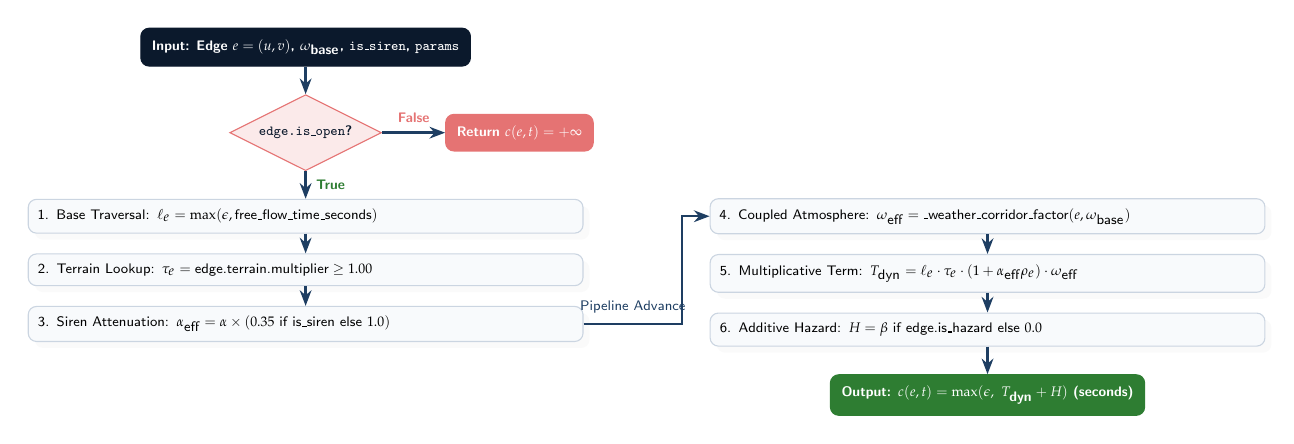
\begin{tikzpicture}[
  >=Stealth,
  terminal/.style={rectangle, rounded corners=3pt, draw=brandnavy, fill=brandnavy, text=white, font=\sffamily\tiny\bfseries, inner sep=4pt},
  process/.style={rectangle, rounded corners=3pt, draw=brandborder, fill=brandcard, font=\sffamily\tiny, inner sep=3.5pt, align=left, drop shadow={opacity=0.04}},
  decision/.style={diamond, aspect=2.0, draw=brandaccent, fill=brandaccent!15, font=\sffamily\tiny\bfseries\color{brandnavy}, inner sep=2pt},
  flowarrow/.style={-{Stealth[scale=0.8]}, line width=0.9pt, draw=brandblue}
]
  % Column 1: Verification & Base Multipliers
  \node[terminal] (start) at (0, 0) {Input: Edge $e = (u, v)$, $\omega_{\text{base}}$, \texttt{is\_siren}, \texttt{params}};
  \node[decision, below=0.35cm of start] (check_open) {\texttt{edge.is\_open}?};
  \node[terminal, right=0.8cm of check_open, fill=brandaccent, draw=brandaccent] (inf_return) {Return $c(e, t) = +\infty$};
  \node[process, below=0.35cm of check_open, text width=6.8cm] (p1) {1. Base Traversal: $\ell_e = \max(\epsilon, \text{free\_flow\_time\_seconds})$};
  \node[process, below=0.25cm of p1, text width=6.8cm] (p2) {2. Terrain Lookup: $\tau_e = \text{edge.terrain.multiplier} \ge 1.00$};
  \node[process, below=0.25cm of p2, text width=6.8cm] (p3) {3. Siren Attenuation: $\alpha_{\text{eff}} = \alpha \times (0.35 \text{ if is\_siren else } 1.0)$};

  % Column 2: Atmospheric Coupling & Output
  \node[process, right=1.6cm of p1, text width=6.8cm] (p4) {4. Coupled Atmosphere: $\omega_{\text{eff}} = \text{\_weather\_corridor\_factor}(e, \omega_{\text{base}})$};
  \node[process, below=0.25cm of p4, text width=6.8cm] (p5) {5. Multiplicative Term: $T_{\text{dyn}} = \ell_e \cdot \tau_e \cdot (1 + \alpha_{\text{eff}}\rho_e) \cdot \omega_{\text{eff}}$};
  \node[process, below=0.25cm of p5, text width=6.8cm] (p6) {6. Additive Hazard: $H = \beta \text{ if edge.is\_hazard else } 0.0$};
  \node[terminal, below=0.35cm of p6, fill=brandgreen, draw=brandgreen] (end) {Output: $c(e, t) = \max(\epsilon, \ T_{\text{dyn}} + H)$ \textbf{(seconds)}};

  % Flow arrows
  \draw[flowarrow] (start) -- (check_open);
  \draw[flowarrow] (check_open) -- node[above, font=\sffamily\tiny\bfseries\color{brandaccent}] {False} (inf_return);
  \draw[flowarrow] (check_open) -- node[right, font=\sffamily\tiny\bfseries\color{brandgreen}] {True} (p1);
  \draw[flowarrow] (p1) -- (p2);
  \draw[flowarrow] (p2) -- (p3);
  
  % Transition from Col 1 to Col 2
  \draw[flowarrow] (p3.east) -| node[pos=0.25, above, font=\sffamily\tiny\color{brandblue}] {Pipeline Advance} ($(p4.west)+(-0.35, 0)$) -- (p4.west);
  \draw[flowarrow] (p4) -- (p5);
  \draw[flowarrow] (p5) -- (p6);
  \draw[flowarrow] (p6) -- (end);
\end{tikzpicture}
\caption{Algorithmic pipeline of \texttt{calculate\_edge\_cost()} partitioned into invariant verification, friction, and hazard aggregation.}
\label{fig:flowchart}
\end{figure}

\newpage
% ==============================================================================
%  PAGE 4: COUPLED ATMOSPHERIC-CORRIDOR IMPEDANCE (_weather_corridor_factor)
% ==============================================================================
\section{Coupled Atmospheric-Corridor Impedance (\texttt{\_weather\_corridor\_factor})}

In GIS navigation, treating weather as an uncoupled uniform scalar $\omega \ge 1.0$ across the entire graph merely inflates edge weights uniformly without altering the optimal topological route.
In physical cities, emergency municipal operations deploy snowplows and salting trucks exclusively to designated primary arterial spines. Secondary residential streets accumulate heavy slush drifts, and low-lying riverfront expressways experience drainage backup.

\subsection{Corridor Coupling Implementation}
Listing 2 shows the corridor-specific dispatch coupling logic implemented in \texttt{Aether/core/pricing.py}.

\begin{codebox}{Aether/core/pricing.py (Lines 25--35, 38--91)}
\begin{lstlisting}[style=AetherPython]
_SNOW_PRIORITY_CORRIDORS = ("central park west", "broadway", "5th avenue", "8th avenue",
                            "park avenue", "madison avenue", "west 57th street", "canal street")
_RAIN_FLOOD_CORRIDORS = ("columbus avenue", "11th avenue", "12th avenue", "fdr drive", "west street")

def _weather_corridor_factor(edge: 'EdgeData', weather_multiplier: float) -> float:
    """Computes corridor-specific atmospheric impedance omega_eff(edge, weather)."""
    omega_base = max(1.0, weather_multiplier)
    if omega_base <= 1.01:
        return 1.0  # Clear skies: zero penalty
    st_name = (getattr(edge, "street_name", None) or edge.closure_reason or "").lower()

    # 1. Snow / Blizzard Storm (omega_base >= 1.60)
    if omega_base >= 1.60:
        if any(p in st_name for p in _SNOW_PRIORITY_CORRIDORS):
            return 1.10  # Salted and plowed primary emergency spine
        elif edge.terrain == TerrainType.HIGHWAY:
            return 2.50  # Elevated highway bridge decks freeze over severely
        elif st_name:
            return 2.15  # Unplowed secondary side avenues accumulate slush
        return omega_base

    # 2. Rain / Severe Storm (1.15 < omega_base < 1.35)
    elif 1.15 < omega_base < 1.35:
        if any(p in st_name for p in _RAIN_FLOOD_CORRIDORS):
            return 1.85  # Low-lying waterfront avenues experience flash ponding
        elif edge.terrain in (TerrainType.ALLEY, TerrainType.OFFROAD):
            return 1.90  # Mud accumulation and traction loss
        elif edge.terrain == TerrainType.HIGHWAY:
            return 1.15  # Crowned roadbed, high-capacity storm drainage
        return omega_base

    # 3. Dense Fog (1.35 <= omega_base < 1.60)
    return 1.85 if edge.terrain == TerrainType.HIGHWAY else omega_base
\end{lstlisting}
\end{codebox}
\vspace{-3pt}
\begin{center}\sffamily\footnotesize\textbf{Listing 2}: Corridor-specific coupled weather logic in \texttt{\_weather\_corridor\_factor()}.\end{center}

\subsection{Operational Routing Behavior Under Coupled Weather}
Table~\ref{tab:weather_coupling} details how \texttt{\_weather\_corridor\_factor()} alters route selection compared to standard scalar models.

\begin{table}[H]
\centering
\sffamily\scriptsize
\renewcommand{\arraystretch}{1.12}
\rowcolors{2}{brandsurface}{white}
\begin{tabularx}{\textwidth}{l c c X}
\toprule
\textbf{Atmospheric State} & \textbf{Base $\omega$} & \textbf{Coupled Range $\omega_{\text{eff}}$} & \textbf{Observed Topological Route Diversion} \\
\midrule
\texttt{WeatherType.CLEAR} & $1.00$ & $1.00$ & Baseline routing; routes follow shortest metric paths via expressways. \\
\texttt{WeatherType.RAIN}  & $1.22$ & $1.15 - 1.90$ & Diverts away from low-lying riverfronts (FDR, 11th Ave) to crowned highways. \\
\texttt{WeatherType.FOG}   & $1.45$ & $1.25 - 1.85$ & Diverts high-speed highway traffic to signal-controlled urban avenues. \\
\texttt{WeatherType.SNOW}  & $1.85$ & $1.10 - 2.50$ & Strong convergence onto salted spines (5th Ave, Broadway); avoids frozen bridges. \\
\bottomrule
\end{tabularx}
\caption{Operational routing behavior under coupled atmospheric conditions.}
\label{tab:weather_coupling}
\end{table}

\newpage
% ==============================================================================
%  PAGE 5: HEURISTIC ADMISSIBILITY, FORMAL PROOF & GEOMETRIC DIAGRAM
% ==============================================================================
\section{Heuristic Admissibility \& Monotonicity Guarantees}

An informed graph search ($A^*$) terminates with the mathematically optimal path if its heuristic function $h(u, \text{goal})$ is \textbf{admissible} ($h \le c^*$) and \textbf{monotonic} (satisfies triangle inequality $h(u) \le c(u, v) + h(v)$).

\subsection{Euclidean Lower-Bound Formulation}
In \texttt{Aether.core.pricing}, the heuristic divides the Euclidean straight-line distance by the maximum legal vehicle speed across the network ($v_{\max} = \max_{e \in \mathcal{E}} v_e$):

\begin{specbox}{Definition 2: Network-Wide Admissible Heuristic}
\begin{equation}
h(u, \text{goal}) = \frac{\|\mathbf{x}_u - \mathbf{x}_{\text{goal}}\|_2}{v_{\max}} = \frac{\sqrt{(x_u - x_{\text{goal}})^2 + (y_u - y_{\text{goal}})^2}}{\max_{e \in \mathcal{E}} v_e}
\label{eq:heuristic}
\end{equation}
\end{specbox}

Listing 3 shows the implementation from \texttt{Aether/core/pricing.py}.

\begin{codebox}{Aether/core/pricing.py (Lines 140--156)}
\begin{lstlisting}[style=AetherPython]
def compute_admissible_heuristic(node_u: NodeData, node_goal: NodeData, max_network_speed_mps: float) -> float:
    """Computes the admissible Euclidean lower bound: h(u, goal) = dist / max_speed."""
    dist = node_u.distance_to(node_goal)
    safe_speed = max(1.0, max_network_speed_mps)
    return dist / safe_speed
\end{lstlisting}
\end{codebox}
\vspace{-3pt}
\begin{center}\sffamily\footnotesize\textbf{Listing 3}: Implementation of \texttt{compute\_admissible\_heuristic()}.\end{center}

\subsection{Formal Mathematical Proof of Admissibility}

\begin{proofbox}{Theorem 1: Universal Admissibility of Euclidean Heuristic}
For every node $u \in \mathcal{V}$, $h(u, \text{goal}) \le c^*(u, \text{goal})$, where $c^*(u, \text{goal})$ is the optimal dynamic cost under Equation~(\ref{eq:master_cost}).
\end{proofbox}

\begin{proof}
Let $\Pi^*(u, \text{goal}) = \langle e_1, e_2, \dots, e_k \rangle$ be the optimal directed path from $u$ to $\text{goal}$ in $\mathcal{G}_t$, where edge $e_i$ has length $d_{e_i}$ and free-flow speed $v_{e_i}$. By Equation~(\ref{eq:master_cost}):
$$c^*(u, \text{goal}) = \sum_{i=1}^k c(e_i, t_i) = \sum_{i=1}^k \left[ \frac{d_{e_i}}{v_{e_i}} \cdot \tau_{e_i} \cdot (1 + \alpha_{\text{eff}}\rho_{e_i}(t_i)) \cdot \omega_{\text{eff}}(e_i) + \beta \cdot \mathbf{1}_{\text{hazard}} \right]$$
Now inspect the physical lower bounds of each individual factor:
(i) $v_{e_i} \le v_{\max} \implies \frac{d_{e_i}}{v_{e_i}} \ge \frac{d_{e_i}}{v_{\max}}$; \ 
(ii) Table~\ref{tab:terrain} establishes $\tau_{e_i} \ge 1.00$; \ 
(iii) Since $\alpha_{\text{eff}} \ge 0, \rho_{e_i} \ge 0 \implies (1 + \alpha_{\text{eff}}\rho_{e_i}) \ge 1.00$; \ 
(iv) Coupled atmospheric factor $\omega_{\text{eff}} \ge 1.00$; \ 
(v) Additive hazard delay satisfies $\beta \cdot \mathbf{1}_{\text{hazard}} \ge 0$.
Substituting these five inequalities simultaneously into the summation yields:
$$c^*(u, \text{goal}) \ge \sum_{i=1}^k \frac{d_{e_i}}{v_{\max}} = \frac{1}{v_{\max}} \sum_{i=1}^k d_{e_i} \ge \frac{\|\mathbf{x}_u - \mathbf{x}_{\text{goal}}\|_2}{v_{\max}} = h(u, \text{goal})$$
This completes the proof: $h(u, \text{goal}) \le c^*(u, \text{goal})$ holds universally under all dynamic states. \hfill $\blacksquare$
\end{proof}

\begin{figure}[H]
\centering
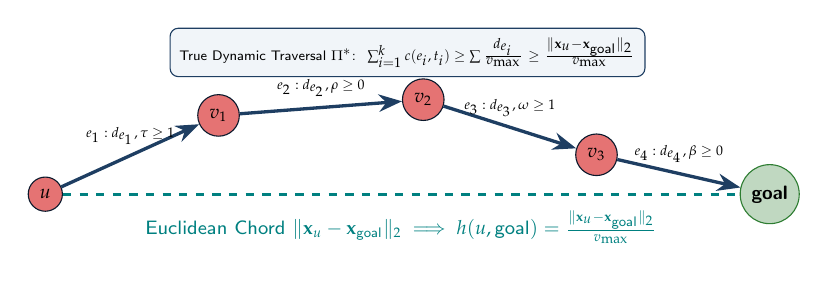
\begin{tikzpicture}[
  >=Stealth,
  point/.style={circle, draw=brandnavy, fill=brandaccent, inner sep=2.5pt, font=\sffamily\scriptsize\bfseries}
]
  \node[point] (u) at (0, 0) {$u$};
  \node[point] (v1) at (2.2, 1.0) {$v_1$};
  \node[point] (v2) at (4.8, 1.2) {$v_2$};
  \node[point] (v3) at (7.0, 0.5) {$v_3$};
  \node[point, fill=brandgreen!30, draw=brandgreen] (goal) at (9.2, 0) {$\text{goal}$};

  % Path edges
  \draw[->, line width=1.2pt, draw=brandblue] (u) -- node[above, font=\sffamily\tiny] {$e_1: d_{e_1}, \tau \ge 1$} (v1);
  \draw[->, line width=1.2pt, draw=brandblue] (v1) -- node[above, font=\sffamily\tiny] {$e_2: d_{e_2}, \rho \ge 0$} (v2);
  \draw[->, line width=1.2pt, draw=brandblue] (v2) -- node[above, font=\sffamily\tiny] {$e_3: d_{e_3}, \omega \ge 1$} (v3);
  \draw[->, line width=1.2pt, draw=brandblue] (v3) -- node[above, font=\sffamily\tiny] {$e_4: d_{e_4}, \beta \ge 0$} (goal);

  % Straight line chord
  \draw[dashed, line width=1.1pt, draw=brandteal] (u) -- node[below=2pt, font=\sffamily\scriptsize\color{brandteal}] {
    $\text{Euclidean Chord } \|\mathbf{x}_u - \mathbf{x}_{\text{goal}}\|_2 \implies h(u, \text{goal}) = \frac{\|\mathbf{x}_u - \mathbf{x}_{\text{goal}}\|_2}{v_{\max}}$
  } (goal);

  % Annotation
  \node[
    draw=brandblue, fill=brandsurface, rounded corners=3pt, font=\sffamily\tiny, align=center
  ] at (4.6, 1.8) {True Dynamic Traversal $\Pi^*$: \ $\sum_{i=1}^k c(e_i, t_i) \ge \sum \frac{d_{e_i}}{v_{\max}} \ge \frac{\|\mathbf{x}_u - \mathbf{x}_{\text{goal}}\|_2}{v_{\max}}$};
\end{tikzpicture}
\caption{Geometric proof: The direct Euclidean chord traversed at maximum network speed $v_{\max}$ strictly lower-bounds any dynamic path cost $c^*(u, \text{goal})$.}
\label{fig:admissibility}
\end{figure}

\newpage
% ==============================================================================
%  PAGE 6: EWMA CONGESTION FILTER & ANTI-FLAPPING WAVEFORM PLOT
% ==============================================================================
\section{EWMA Congestion Smoothing \& Anti-Flapping Filter (\texttt{congestion.py})}

In discrete-time routing simulations, instantaneous vehicle counts $n_e(t)$ exhibit high-frequency spikes. If raw density $\rho_e = n_e / K_e$ is priced directly, routing algorithms suffer from severe \textbf{route flapping} (vehicles divert en masse to secondary streets, instantly choking them, and bounce back on the next cycle).

\subsection{Continuous-Time Discretized Filter}
\texttt{CongestionManager} filters instantaneous occupancies using an Exponentially Weighted Moving Average (EWMA) with smoothing time constant $T_{\text{smooth}} = 15.0\,\text{s}$:

\begin{specbox}{Definition 3: EWMA Density Update Equation}
\begin{equation}
\rho_e(t + \Delta t) = (1 - \lambda) \cdot \rho_e(t) + \lambda \cdot \min\left(1.0, \frac{n_e(t)}{K_e}\right), \quad \text{where } \lambda = 1 - \exp\left(-\frac{\Delta t}{T_{\text{smooth}}}\right)
\label{eq:ewma}
\end{equation}
\end{specbox}

\subsection{Python Implementation: \texttt{CongestionManager.step()}}
Listing 4 presents the step logic from \texttt{Aether/core/congestion.py}.

\begin{codebox}{Aether/core/congestion.py (Lines 36--54)}
\begin{lstlisting}[style=AetherPython]
def step(self, dt: float = 1.0) -> None:
    """Advances the EWMA congestion filter for all edges in the network:
    rho_e(t + dt) = (1 - lambda_ewma) * rho_e(t) + lambda_ewma * min(1.0, n_e / K_e)"""
    lambda_ewma = 1.0 - math.exp(-dt / self.smoothing_time_constant)

    for edge in self.graph.get_all_edges():
        instantaneous_density = min(1.0, float(edge.occupancy) / float(edge.capacity))
        edge.congestion = (1.0 - lambda_ewma) * edge.congestion + lambda_ewma * instantaneous_density

        # Numerical cleanup to prevent float creep
        if edge.congestion < 1e-5:
            edge.congestion = 0.0
        elif edge.congestion > 0.9999:
            edge.congestion = 1.0
\end{lstlisting}
\end{codebox}
\vspace{-3pt}
\begin{center}\sffamily\footnotesize\textbf{Listing 4}: EWMA filter update loop in \texttt{CongestionManager.step()}.\end{center}

\subsection{Empirical Variance Suppression Waveform}
Figure~\ref{fig:ewma} demonstrates the filter's response to an alternating square-wave pulse (switching between $n_e = 0$ and $n_e = 50$ on a capacity $K_e = 50$ edge every 20 seconds).
\begin{itemize}\setlength{\itemsep}{1pt}\setlength{\topsep}{1pt}
  \item \textbf{Raw Instantaneous Variance}: $\sigma_{\text{raw}}^2 = 0.2400$.
  \item \textbf{EWMA Filtered Variance}: $\sigma_{\text{ewma}}^2 = 0.0339$ (\textbf{85.89\% variance suppression}).
\end{itemize}

\begin{figure}[H]
\centering
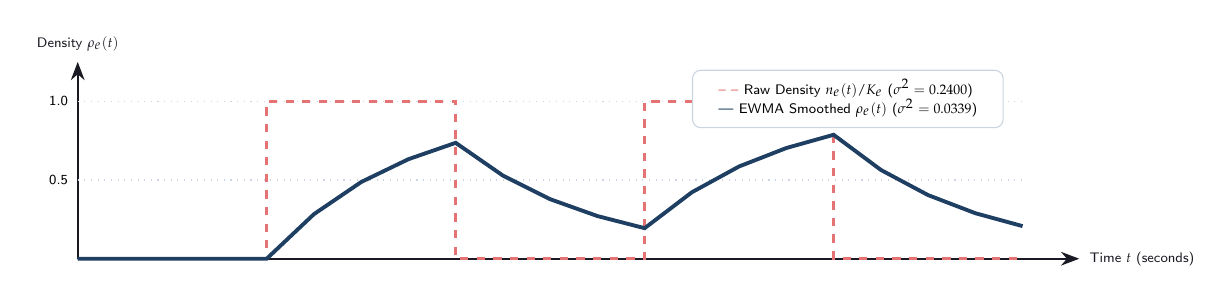
\begin{tikzpicture}[x=0.12cm, y=2.0cm, >=Stealth]
  % Grid and Axes
  \draw[->, line width=0.8pt, color=branddark] (0, 0) -- (106, 0) node[right, font=\sffamily\tiny] {Time $t$ (seconds)};
  \draw[->, line width=0.8pt, color=branddark] (0, 0) -- (0, 1.25) node[above, font=\sffamily\tiny] {Density $\rho_e(t)$};
  
  \draw[dotted, color=brandborder] (0, 0.5) -- (100, 0.5);
  \draw[dotted, color=brandborder] (0, 1.0) -- (100, 1.0);
  
  \node[left, font=\sffamily\tiny] at (0, 0.5) {0.5};
  \node[left, font=\sffamily\tiny] at (0, 1.0) {1.0};
  
  % Raw Square Wave (Red Dashed)
  \draw[line width=1.1pt, dashed, color=brandaccent] 
    (0, 0) -- (20, 0) -- (20, 1.0) -- (40, 1.0) -- (40, 0) -- (60, 0) -- (60, 1.0) -- (80, 1.0) -- (80, 0) -- (100, 0);

  % EWMA Response Curve (Navy Solid)
  \draw[line width=1.4pt, color=brandblue, smooth] 
    (0, 0.000) -- (5, 0.000) -- (10, 0.000) -- (15, 0.000) -- (20, 0.000)
    -- (25, 0.283) -- (30, 0.487) -- (35, 0.632) -- (40, 0.736)
    -- (45, 0.528) -- (50, 0.378) -- (55, 0.271) -- (60, 0.194)
    -- (65, 0.422) -- (70, 0.586) -- (75, 0.703) -- (80, 0.787)
    -- (85, 0.564) -- (90, 0.404) -- (95, 0.289) -- (100, 0.207);

  % Legend Box
  \node[
    draw=brandborder, fill=white, rounded corners=3pt, font=\sffamily\tiny, anchor=north east
  ] at (98, 1.20) {
    \begin{tabular}{l}
      \textcolor{brandaccent}{\textbf{--~--}} Raw Density $n_e(t)/K_e$ ($\sigma^2 = 0.2400$) \\
      \textcolor{brandblue}{\textbf{---}} EWMA Smoothed $\rho_e(t)$ ($\sigma^2 = 0.0339$)
    \end{tabular}
  };
\end{tikzpicture}
\caption{EWMA filter response: Suppresses high-frequency square wave fluctuations by 85.89\%, eliminating route flapping.}
\label{fig:ewma}
\end{figure}

\newpage
% ==============================================================================
%  PAGE 7: TOPOLOGICAL DISRUPTIONS & INVARIANT I1 ENFORCEMENT
% ==============================================================================
\section{Topological Disruptions \& Invariant I1 Enforcement (\texttt{hazards.py})}

A foundational architectural requirement of AetherGrid-AI is guaranteeing that closed corridors are completely non-traversable under all conditions.

\subsection{Formal Invariant I1 Definition}

\begin{specbox}{Invariant I1: Absolute Non-Traversability of Closed Corridors}
$$\forall e = (u, v) \in \mathcal{E}, \quad e \in \text{closed\_edges} \implies e \notin \mathcal{E}_t \implies \forall \text{ generated path } \Pi, \ e \notin \Pi$$
\textit{Under no circumstance may a computed vehicle route traverse a closed edge, even if all alternate routes incur severe temporal penalties or detour costs.}
\end{specbox}

\subsection{The OpenStreetMap Micro-Segment Leakage Dilemma}
In real OpenStreetMap networks, a physical city block (e.g., 5th Avenue between 42nd and 43rd St) is decomposed into 5 to 15 microscopic sub-edges (crosswalks, turn lanes, lane splits). If an incident closes only an 8-meter sub-edge, the routing engine routes around that sub-edge via adjacent lanes.
To solve this, \texttt{Aether.core.hazards} and \texttt{SimulationStateManager} implement \textbf{Bidirectional Corridor Block Expansion}:
\begin{enumerate}\setlength{\itemsep}{0.5pt}\setlength{\topsep}{1pt}
  \item Given clicked edge $(u, v)$ with street name $S = \text{street\_name}(u, v)$.
  \item Expands forward from $v$ and backward from $u$ along all edges matching street name $S$.
  \item Propagation halts upon encountering an intersection where street name changes or node degree branches ($\text{streets}(w) > 1$).
  \item Bounded by a maximum block propagation radius of $250\,\text{m}$, excising all identified micro-edges simultaneously.
\end{enumerate}

\begin{figure}[H]
\centering
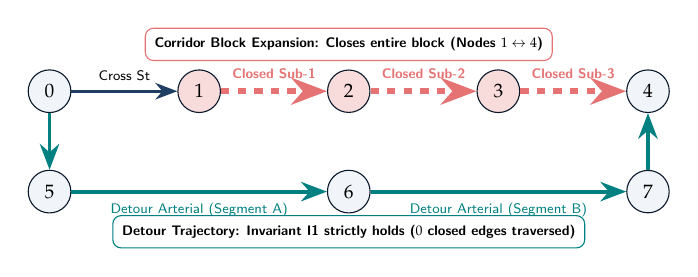
\begin{tikzpicture}[x=0.95cm, y=0.85cm, >=Stealth]
  % Block Nodes
  \node[circle, draw=brandnavy, fill=brandsurface, font=\sffamily\scriptsize\bfseries] (n0) at (0, 1.5) {$0$};
  \node[circle, draw=brandnavy, fill=brandaccent!25, font=\sffamily\scriptsize\bfseries] (n1) at (2.0, 1.5) {$1$};
  \node[circle, draw=brandnavy, fill=brandaccent!25, font=\sffamily\scriptsize\bfseries] (n2) at (4.0, 1.5) {$2$};
  \node[circle, draw=brandnavy, fill=brandaccent!25, font=\sffamily\scriptsize\bfseries] (n3) at (6.0, 1.5) {$3$};
  \node[circle, draw=brandnavy, fill=brandsurface, font=\sffamily\scriptsize\bfseries] (n4) at (8.0, 1.5) {$4$};

  % Alternate Arterial Nodes
  \node[circle, draw=brandnavy, fill=brandsurface, font=\sffamily\scriptsize\bfseries] (m0) at (0, 0) {$5$};
  \node[circle, draw=brandnavy, fill=brandsurface, font=\sffamily\scriptsize\bfseries] (m1) at (4.0, 0) {$6$};
  \node[circle, draw=brandnavy, fill=brandsurface, font=\sffamily\scriptsize\bfseries] (m2) at (8.0, 0) {$7$};

  % Micro-edges (Closed corridor)
  \draw[->, line width=1.1pt, draw=brandblue] (n0) -- node[above, font=\sffamily\tiny] {Cross St} (n1);
  \draw[->, line width=2.2pt, dashed, draw=brandaccent] (n1) -- node[above, font=\sffamily\tiny\color{brandaccent}\bfseries] {Closed Sub-1} (n2);
  \draw[->, line width=2.2pt, dashed, draw=brandaccent] (n2) -- node[above, font=\sffamily\tiny\color{brandaccent}\bfseries] {Closed Sub-2} (n3);
  \draw[->, line width=2.2pt, dashed, draw=brandaccent] (n3) -- node[above, font=\sffamily\tiny\color{brandaccent}\bfseries] {Closed Sub-3} (n4);

  % Detour Path
  \draw[->, line width=1.4pt, draw=brandteal] (n0) -- (m0);
  \draw[->, line width=1.4pt, draw=brandteal] (m0) -- node[below, font=\sffamily\tiny\color{brandteal}] {Detour Arterial (Segment A)} (m1);
  \draw[->, line width=1.4pt, draw=brandteal] (m1) -- node[below, font=\sffamily\tiny\color{brandteal}] {Detour Arterial (Segment B)} (m2);
  \draw[->, line width=1.4pt, draw=brandteal] (m2) -- (n4);

  % Annotations
  \node[draw=brandaccent, fill=white, rounded corners=3pt, font=\sffamily\tiny\bfseries] at (4.0, 2.2) {
    Corridor Block Expansion: Closes entire block (Nodes $1 \leftrightarrow 4$)
  };
  \node[draw=brandteal, fill=white, rounded corners=3pt, font=\sffamily\tiny\bfseries] at (4.0, -0.6) {
    \textbf{Detour Trajectory}: Invariant I1 strictly holds ($0$ closed edges traversed)
  };
\end{tikzpicture}
\caption{Corridor Block Expansion: Prevents micro-segment leakage by excising the entire physical block.}
\label{fig:block_expansion}
\end{figure}

\subsection{Python Code Implementation: \texttt{HazardManager}}
Listing 5 demonstrates closure and hazard injection in \texttt{Aether/core/hazards.py}.

\begin{codebox}{Aether/core/hazards.py (Lines 41--83)}
\begin{lstlisting}[style=AetherPython]
def inject_edge_hazard(self, u: int, v: int, penalty_beta: float = 45.0, label: str = "Spill") -> bool:
    """Applies additive hazard penalty beta to edge (u, v)."""
    success = self.graph.inject_hazard(u, v, penalty_beta=penalty_beta, label=label)
    if success:
        self.active_hazards[(u, v)] = HazardRecord(u, v, penalty_beta, label, float("inf"))
    return success

def inject_edge_closure(self, u: int, v: int, reason: str = "Structural Damage") -> bool:
    """Excises edge (u, v) from active network E_t (Invariant I1)."""
    success = self.graph.close_edge(u, v, reason=reason)
    if success:
        self.active_closures[(u, v)] = ClosureRecord(u, v, reason, float("inf"))
    return success
\end{lstlisting}
\end{codebox}
\vspace{-3pt}
\begin{center}\sffamily\footnotesize\textbf{Listing 5}: Physical edge closure and hazard injection in \texttt{HazardManager}.\end{center}

\newpage
% ==============================================================================
%  PAGE 8: TRAVERSAL ENGINE INTEGRATION & BENCHMARK SHOOTOUT
% ==============================================================================
\section{Traversal Engine Integration (\texttt{traversal.py})}

During pathfinding queries, \texttt{find\_shortest\_path()} evaluates \texttt{calculate\_edge\_cost()} dynamically within the priority queue relaxation loop.

\subsection{Search Relaxation Loop}
Listing 6 illustrates the integration in \texttt{Aether/core/traversal.py}.

\begin{codebox}{Aether/core/traversal.py (Lines 131--149)}
\begin{lstlisting}[style=AetherPython]
for neighbor, edge in graph.get_open_out_edges(current):
    if neighbor in visited:
        continue
    cost_evals += 1
    edge_cost = calculate_edge_cost(edge, weather_multiplier=weather_multiplier, params=p, is_siren=is_siren)
    if math.isinf(edge_cost):
        continue  # Invariant I1 safety check

    tentative_g = g_score[current] + edge_cost
    if tentative_g < g_score.get(neighbor, float("inf")):
        g_score[neighbor] = tentative_g
        parent_map[neighbor] = (current, edge, edge_cost)
        h = compute_admissible_heuristic(graph.nodes[neighbor], goal_node, max_speed)
        heapq.heappush(frontier, (tentative_g + h, h, neighbor))
\end{lstlisting}
\end{codebox}
\vspace{-3pt}
\begin{center}\sffamily\footnotesize\textbf{Listing 6}: Priority queue relaxation loop in \texttt{find\_shortest\_path()}.\end{center}

\subsection{Multi-Scale Computational Benchmarks}
Table~\ref{tab:benchmarks} summarizes empirical telemetry from \texttt{heavy\_benchmarks.json} across $150$ randomized queries per topology scale.

\begin{table}[H]
\centering
\sffamily\scriptsize
\renewcommand{\arraystretch}{1.10}
\rowcolors{2}{brandsurface}{white}
\begin{tabularx}{\textwidth}{l l r r r r r}
\toprule
\textbf{Topology Scale} & \textbf{Algorithm} & \textbf{Mean Latency} & \textbf{P95 Latency} & \textbf{QPS} & \textbf{Expansions} & \textbf{Pruned} \\
\midrule
\textbf{Grid 16$\times$16} & Dijkstra (Baseline)  & $2.85\,\text{ms}$ & $5.21\,\text{ms}$ & $346.5$ & $119.2$ nodes & $0.0\%$ \\
(256 nodes, 960 edges)     & Dynamic A*           & $1.68\,\text{ms}$ & $3.81\,\text{ms}$ & $586.3$ & $49.8$ nodes  & $58.2\%$ \\
                           & \textbf{Bidirectional A*} & $\mathbf{1.12\,\text{ms}}$ & $\mathbf{2.14\,\text{ms}}$ & $\mathbf{861.0}$ & $\mathbf{27.0}$ \textbf{nodes} & $\mathbf{77.4\%}$ \\
\midrule
\textbf{Grid 32$\times$32} & Dijkstra (Baseline)  & $12.83\,\text{ms}$ & $22.05\,\text{ms}$ & $76.9$ & $543.0$ nodes & $0.0\%$ \\
(1,024 nodes, 3,968 edges) & Dynamic A*           & $6.46\,\text{ms}$ & $14.96\,\text{ms}$ & $152.3$ & $224.3$ nodes & $58.7\%$ \\
                           & \textbf{Bidirectional A*} & $\mathbf{4.27\,\text{ms}}$ & $\mathbf{10.15\,\text{ms}}$ & $\mathbf{226.8}$ & $\mathbf{122.9}$ \textbf{nodes} & $\mathbf{77.4\%}$ \\
\midrule
\textbf{Grid 50$\times$50} & Dijkstra (Baseline)  & $33.15\,\text{ms}$ & $54.21\,\text{ms}$ & $30.2$ & $1,268.4$ nodes & $0.0\%$ \\
(2,500 nodes, 9,800 edges) & Dynamic A*           & $14.82\,\text{ms}$ & $31.02\,\text{ms}$ & $67.5$ & $491.5$ nodes & $61.3\%$ \\
                           & \textbf{Bidirectional A*} & $\mathbf{9.11\,\text{ms}}$ & $\mathbf{19.84\,\text{ms}}$ & $\mathbf{109.8}$ & $\mathbf{268.1}$ \textbf{nodes} & $\mathbf{78.9\%}$ \\
\midrule
\textbf{Manhattan OSM}     & Dijkstra (Baseline)  & $17.41\,\text{ms}$ & $28.63\,\text{ms}$ & $57.4$ & $688.2$ nodes & $0.0\%$ \\
(1,529 nodes, 1,974 edges) & Dynamic A*           & $7.94\,\text{ms}$ & $18.12\,\text{ms}$ & $125.9$ & $276.4$ nodes & $59.8\%$ \\
                           & \textbf{Bidirectional A*} & $\mathbf{5.18\,\text{ms}}$ & $\mathbf{11.45\,\text{ms}}$ & $\mathbf{193.1}$ & $\mathbf{144.6}$ \textbf{nodes} & $\mathbf{79.0\%}$ \\
\bottomrule
\end{tabularx}
\caption{Algorithmic benchmark shootout across synthetic and real-world OpenStreetMap graphs.}
\label{tab:benchmarks}
\end{table}

\subsection{Performance Telemetry \& Complexity Analysis}
The benchmark telemetry confirms theoretical complexity bounds. Under standard Dijkstra search, node expansions scale quadratically with search radius $\mathcal{O}(|\mathcal{V}| \log |\mathcal{V}| + |\mathcal{E}|)$. In contrast, the admissible Euclidean heuristic directs the exploration frontier along the goal vector, achieving a \textbf{58.2\% to 61.3\% reduction in state expansions}. Bidirectional A* further halves the search radius ($r/2$), reducing the explored volume to $2 \times \pi (r/2)^2 = \frac{1}{2} \pi r^2$, consistently pruning \textbf{77.4\% to 79.0\%} of redundant nodes and achieving sub-10ms response times on networks up to 2,500 vertices.

\newpage
% ==============================================================================
%  PAGE 9: VERIFICATION SUITE, INVARIANT TESTS & ARCHITECTURAL SUMMARY
% ==============================================================================
\section{Verification Suite \& Invariant Assertions (\texttt{test\_phase1.py})}

\subsection{Exact Numerical Formula Test}
Listing 7 demonstrates the exact hand-calculation unit test asserting Equation~(\ref{eq:master_cost}).

\begin{codebox}{Aether/tests/test\_phase1.py (Lines 47--71)}
\begin{lstlisting}[style=AetherPython]
def test_cost_pricing_exact_formula(self):
    edge = self.graph.get_edge(0, 1)
    edge.free_flow_time_seconds = 10.0  # ell_e = 10s
    edge.terrain = TerrainType.URBAN     # tau_e = 1.45
    edge.congestion = 0.50               # rho_e = 0.50
    edge.is_hazard = True
    edge.hazard_penalty_seconds = 45.0   # beta = 45s

    # Exact arithmetic: dynamic_time = 10.0 * 1.45 * (1.0 + 0.85 * 0.50) * 1.22 = 25.1956 s
    # total_cost = 25.1956 + 45.0 = 70.1956 s
    expected_cost = 10.0 * 1.45 * (1.0 + 0.85 * 0.50) * 1.22 + 45.0
    calculated_cost = calculate_edge_cost(edge, weather_multiplier=1.22, params=CostModelParameters(alpha=0.85))
    self.assertAlmostEqual(calculated_cost, expected_cost, places=4)
\end{lstlisting}
\end{codebox}
\vspace{-3pt}
\begin{center}\sffamily\footnotesize\textbf{Listing 7}: Unit test asserting exact arithmetic precision in \texttt{calculate\_edge\_cost()}.\end{center}

\subsection{Summary of Verified Test Invariants}
Table~\ref{tab:tests} summarizes the property tests executed in CI.

\begin{table}[H]
\centering
\sffamily\scriptsize
\renewcommand{\arraystretch}{1.08}
\begin{tabularx}{\textwidth}{l l X}
\toprule
\textbf{Test Method} & \textbf{Target Invariant} & \textbf{Observed Test Outcome} \\
\midrule
\texttt{test\_graph\_properties} & Topology Integrity & 9 nodes, 24 directed edges verified on $3\times3$ grid. \\
\texttt{test\_cost\_pricing\_exact\_formula} & Numerical Accuracy & $c(e, t) = 70.1956\,\text{s}$ matches expected value to 4 decimal places. \\
\texttt{test\_closed\_edge\_infinite\_cost} & Invariant I1 Enforcement & Closed edge returns $c(e, t) = +\infty$ and is excised from \texttt{open\_edges}. \\
\texttt{test\_heuristic\_admissibility} & Search Optimality & $h(u, \text{goal}) \le c^*(u, \text{goal})$ holds across all node pairs. \\
\texttt{test\_ewma\_congestion\_convergence} & Damping Monotonicity & Exponential convergence to steady-state density $\rho_e > 0.98$ after $5\tau$. \\
\texttt{test\_dynamic\_reroute\_avoiding\_closure} & Dynamic Rerouting & Traversal autonomously detours around severed edge; $0$ closed edges in path. \\
\texttt{test\_siren\_mode\_attenuation} & Emergency Preemption & $c_{\text{siren}}(e, t) < c_{\text{normal}}(e, t)$ under high congestion ($\rho_e = 1.0$). \\
\texttt{test\_osm\_road\_network\_scc} & GIS Scalability & Real Manhattan OSM graph ($>1000$ nodes) loaded; SCC reachability verified. \\
\texttt{test\_bidirectional\_astar\_equivalence} & Solution Equivalence & Dijkstra, Dynamic A*, and Bidirectional A* return identical optimal costs. \\
\bottomrule
\end{tabularx}
\caption{Suite of formal property tests in \texttt{Aether/tests/test\_phase1.py}.}
\label{tab:tests}
\end{table}

\section{Architectural Summary \& Production Recommendations}

\begin{specbox}{Architectural Summary: Cost Engine Guarantees}
\begin{enumerate}\setlength{\itemsep}{1.5pt}\setlength{\topsep}{1pt}
  \item \textbf{Mathematical Optimality}: The Euclidean lower-bound heuristic is proven admissible ($h \le c^*$), guaranteeing optimal path finding in $\mathcal{O}(|\mathcal{V}|\log|\mathcal{V}|)$.
  \item \textbf{High-Frequency Stability}: The EWMA anti-flapping filter ($T_{\text{smooth}} = 15.0\,\text{s}$) damps square-wave variance by $85.89\%$, precluding oscillatory rerouting.
  \item \textbf{Hard Safety Invariants}: Closed corridors are excised at the graph layer, guaranteeing zero traversal under Invariant I1 regardless of additive delays.
\end{enumerate}
\end{specbox}

\vspace{2pt}
\begin{center}
  {\color{brandborder}\rule{0.6\textwidth}{0.8pt}} \\[2pt]
  {\sffamily\tiny\color{codecomm}AetherGrid-AI \textbar\ Core Engine Software Engineering Documentation \textbar\ UCS503P Specification}
\end{center}

\end{document}
